% Provenance (never printed): see sources/outline_sources.md (Year 2: mid-latitude cyclones and
% fronts; jets and Rossby waves, descriptive; tropical cyclones; numerical weather prediction,
% principle). Definitions after the NWS glossary and UCAR; cyclogenesis conditions after the NOAA
% AOML FAQ; potential intensity after Gilford (2021, pyPI); conveyor belts after Raveh-Rubin and
% Catto (2019); blocking after Wang and others (2026); predictability after Krishnamurthy (2019),
% Selz and others (2022) and ECMWF. The Lorenz system from figdata/bachelor-2/weather.py; the
% fronts, waves and storms of the examples, exercises and problem are invented, their values
% computed in the Book 4 scratch calculator calc/ch22.py.
\chapter{Sistemas meteorológicos}\label{ch:b2:weather-systems}

Una predicción a cuatro días es hoy tan precisa como lo era una predicción a un día hace treinta
años, y cada década ha añadido aproximadamente un día de predicción útil. Sin embargo, ninguna predicción del
tiempo de un día dado, en un lugar dado, es fiable mucho más allá de diez días, y unos ordenadores mejores
no bastarán por sí solos para alejar mucho ese límite: la atmósfera amplifica sus propias pequeñas incertidumbres. Este
capítulo describe los sistemas meteorológicos que siguen las predicciones, los frentes y las depresiones de las
latitudes medias, las ondas de la corriente en chorro y los ciclones tropicales, y después la manera en que se
predicen y por qué la predicción tiene que detenerse en algún punto.
% ledger: mo:accuracy, bauer:day-per-decade, krish19:predictability

\begin{recall}
\textbf{De los volúmenes escolares}: las masas de aire, los frentes, los frentes fríos y cálidos, las depresiones y
los anticiclones, las isobaras y las predicciones meteorológicas; el ciclón tropical, su ojo y su pared del ojo, la
escala de Saffir--Simpson. \textbf{Del volumen de primer año}: la fuerza del gradiente de presión, el
parámetro de Coriolis $f = 2\Omega\sin\varphi$, el equilibrio geostrófico, los ciclones y los anticiclones, las
tres células, los vientos del oeste y las corrientes en chorro. \textbf{De los libros de física}: las máquinas térmicas
y el rendimiento de un ciclo de Carnot. \textbf{Del \cref{ch:b2:atmospheric-thermodynamics}}:
la saturación, la \omterm{def:b2:atmospheric-thermodynamics:moist-adiabat}{adiabática húmeda}, $\theta_e$, la \omterm{def:b2:atmospheric-thermodynamics:instability}{inestabilidad condicional} y la CAPE.
\end{recall}

\section{Los frentes}\label{sec:b2:weather-systems:fronts}

Los volúmenes escolares dibujaban los frentes como líneas en un mapa. Un frente es la línea donde una superficie inclinada
que separa dos masas de aire corta el suelo, y su tiempo procede de esa inclinación.

\begin{definition}[Superficie frontal; frente estacionario; frente ocluido]\label{def:b2:weather-systems:fronts}
La \emph{superficie frontal}\index{superficie frontal} de un frente es la superficie inclinada que separa
las dos masas de aire, con la más densa y fría debajo, en forma de cuña; el frente del mapa es su
intersección con el suelo. Un \emph{frente estacionario}\index{frente estacionario} es un frente
que se desplaza muy despacio o no se desplaza. Un \emph{frente ocluido}\index{frente ocluido} es un
compuesto de dos frentes, formado cuando un frente frío alcanza a un frente cálido o estacionario.
\end{definition}
% ledger: nws4:front, nws4:stationary, nws4:occluded

Un \omterm{def:b2:weather-systems:fronts}{frente estacionario} se forma cuando ninguna de las dos masas de aire puede empujar a la otra, porque los vientos soplan a lo largo del
frente en lugar de atravesarlo; puede permanecer días, nuboso y húmedo, antes de volver a moverse como frente frío
o cálido. En un mapa alterna los triángulos azules de un frente frío, que apuntan hacia el
aire cálido, con los semicírculos rojos de un frente cálido, que apuntan hacia el aire frío. Un \omterm{def:b2:weather-systems:fronts}{frente
ocluido} se dibuja en violeta con ambos símbolos del mismo lado. Cuando el aire de detrás del frente frío
es el más frío, se desliza bajo el frente cálido y lo levanta en altura: una oclusión fría; cuando el aire
de delante del frente cálido es el más frío, el frente frío asciende por encima de él: una oclusión cálida.
% ledger: ucar4:stationary-occluded, nws4:occluded

¿Qué inclinación tiene una \omterm{def:b2:weather-systems:fronts}{superficie frontal}? La respuesta une el equilibrio hidrostático al equilibrio
geostrófico del volumen de primer año.

\begin{proposition}[Pendiente de una superficie frontal]\label{prop:b2:weather-systems:slope}
Sea una \omterm{def:b2:weather-systems:fronts}{superficie frontal} que separa aire frío a la temperatura $T_c$ de aire cálido a $T_w$, con
vientos geostróficos $v_c$ y $v_w$ a lo largo del frente. Tómese el eje $x$ a través del frente hacia el
aire frío y el eje $y$ a lo largo de él, de modo que $(x, y, z)$ sea directo. Entonces la \omterm{def:b2:weather-systems:fronts}{superficie
frontal} se eleva hacia el aire frío con la pendiente
\[
  \tan\alpha \approx \frac{f\,\bar T\,(v_c - v_w)}{g\,(T_w - T_c)},
\]
donde $\bar T$ es la temperatura media. Una \omterm{def:b2:weather-systems:fronts}{superficie frontal} en equilibrio necesita un salto del viento
a lo largo de ella, $v_c > v_w$: el viento gira ciclónicamente a través del frente.
\end{proposition}

\begin{proof}
La presión es continua a través de la \omterm{def:b2:weather-systems:fronts}{superficie frontal}, así que su variación a lo largo de la superficie es la
misma calculada a uno u otro lado: $\partial_x p_c\,\mathrm{d}x + \partial_z p_c\,\mathrm{d}z =
\partial_x p_w\,\mathrm{d}x + \partial_z p_w\,\mathrm{d}z$. A cada lado, $\partial_z p = -\rho g$
(equilibrio hidrostático) y $\partial_x p = \rho f v$ (equilibrio geostrófico). Por tanto
$\rho_c f v_c\,\mathrm{d}x - \rho_c g\,\mathrm{d}z = \rho_w f v_w\,\mathrm{d}x - \rho_w
g\,\mathrm{d}z$, y
\[
  \frac{\mathrm{d}z}{\mathrm{d}x} = \frac{f(\rho_c v_c - \rho_w v_w)}{g(\rho_c - \rho_w)} .
\]
A la misma presión, $\rho \propto 1/T$, así que $\rho_c - \rho_w \approx \bar\rho\,(T_w -
T_c)/\bar T$; en el numerador puede despreciarse la pequeña diferencia de las densidades, lo que
da la fórmula. El aire frío está debajo, así que la superficie se eleva hacia él, $\mathrm{d}z/
\mathrm{d}x > 0$, y $v_c > v_w$. Con $x$ hacia el aire frío, la vorticidad relativa
$\partial v/\partial x$ a través del frente es entonces positiva: ciclónica.
\end{proof}

\begin{example}[Una pendiente típica]\label{ex:b2:weather-systems:slope}
A \ang{45} N, $f = \qty{1.03e-4}{s^{-1}}$. A través de un frente con $\bar T = \qty{280}{K}$, un
contraste de temperatura de \qty{5}{K} y un viento que cambia \qty{10}{m/s} a lo largo de él, $\tan\alpha
= 1.03 \times 10^{-4} \times 280 \times 10/(9.81 \times 5) = 0.0059$, aproximadamente 1 por cada 170: la
\omterm{def:b2:weather-systems:fronts}{superficie frontal} alcanza una altura de \qty{1}{km} a unos \qty{170}{km} del frente en el suelo.
Un salto de viento más brusco da una superficie más empinada; un contraste de temperatura mayor, una más suave.
\end{example}

Los frentes reales tienen pendientes de este orden, y la cuña poco inclinada explica su tiempo. Por delante de un
frente cálido, el aire cálido asciende por una pendiente suave a lo largo de cientos de kilómetros: llegan primero las nubes altas,
cirros y cirrostratos, luego los altostratos, y las nubes se espesan y bajan hasta que
empieza a llover cerca del frente. Un frente frío, más empinado y más rápido, hasta el doble de rápido que un frente
cálido, levanta bruscamente el aire cálido: cúmulos y cumulonimbos, chubascos, rachas y una caída repentina
de la temperatura, con una presión que deja de bajar y empieza a subir al paso del frente. Un frente
donde el aire cálido desciende por la \omterm{def:b2:weather-systems:fronts}{superficie frontal} en lugar de ascender por ella se llama catafrente.
% ledger: ucar:warm-front, ucar:cold-front, nws4:front

\begin{omfigure}
\centering
\begin{tikzpicture}[font=\scriptsize, >=Stealth, x=1cm, y=1cm]
% air masses
\fill[omCold!12] (0,0) -- (0,3.4) .. controls (1.6,2.2) and (3.2,0.8) .. (4,0) -- cycle;
\fill[omCold!12] (9.6,0) .. controls (11,0.6) and (12.6,1.5) .. (14,2.4) -- (14,0) -- cycle;
\fill[omWarm!8] (4,0) .. controls (3.2,0.8) and (1.6,2.2) .. (0,3.4) -- (0,4.8) -- (14,4.8)
  -- (14,2.4) .. controls (12.6,1.5) and (11,0.6) .. (9.6,0) -- cycle;
% frontal surfaces
\draw[omCold, thick] (4,0) .. controls (3.2,0.8) and (1.6,2.2) .. (0,3.4);
\draw[omWarm, thick] (9.6,0) .. controls (11,0.6) and (12.6,1.5) .. (14,2.4);
% clouds
\fill[black!18, draw=black!45] (3.75,0.5) .. controls (3.5,1.8) and (3.7,3.2) .. (3.9,3.9)
  .. controls (3.2,4.15) and (3.0,4.5) .. (3.4,4.6) -- (5.8,4.6) .. controls (6.1,4.45) and
  (5.7,4.15) .. (5.1,3.9) .. controls (5.3,3.0) and (5.4,1.6) .. (5.05,0.5) -- cycle;
\node[align=center] at (4.45,2.6) {cumulo-\\nimbos};
\fill[black!15, draw=black!40] (9.6,0.35) .. controls (10.4,0.75) and (11.2,1.05) .. (11.9,1.25)
  -- (11.9,1.75) .. controls (11,1.6) and (10.2,1.35) .. (9.4,0.95) -- cycle;
\node at (10.75,1.25) [rotate=21] {nimbostratos};
\fill[black!10, draw=black!35] (11.9,1.35) .. controls (12.3,1.55) and (12.7,1.75) .. (13.0,1.9)
  -- (13.0,2.25) .. controls (12.6,2.1) and (12.2,1.95) .. (11.9,1.85) -- cycle;
\node[anchor=south] at (12.45,2.15) {altostratos};
\draw[black!40, line width=1.6pt] (12.9,2.75) -- (13.9,3.05);
\node[anchor=south] at (13.35,3.05) {cirrostratos};
\foreach \x in {12.2,12.7,13.2,13.7} {\draw[black!40, thick] (\x,3.95) .. controls (\x+0.15,4.05) .. (\x+0.35,3.9);}
\node[anchor=south] at (13.0,4.05) {cirros};
% rain
\foreach \x in {3.95,4.25,4.55,4.85} {\draw[omCold!70, dashed] (\x,0.45) -- (\x-0.12,0.02);}
\foreach \x in {9.8,10.2,10.6,11.0,11.4} {\draw[omCold!70, dashed] (\x,0.55) -- (\x-0.12,0.02);}
% ground and labels
\draw[thick] (0,0) -- (14,0);
\node at (1.2,0.8) {aire frío};
\node at (7.0,2.4) {sector cálido};
\node at (12.8,0.55) {aire frío};
\node[anchor=north, omCold] at (4,-0.05) {frente frío};
\node[anchor=north, omWarm] at (9.6,-0.05) {frente cálido};
\draw[->, thick] (6.0,0.55) -- (7.2,0.55) node[right] {\shortstack[l]{los frentes\\avanzan al este}};
\draw[->, black!60] (5.8,1.1) .. controls (7.0,1.4) and (9.5,2.0) .. (12.2,3.3);
\node[black!60, rotate=13] at (8.4,2.0) {el aire cálido sube};
\end{tikzpicture}
\par\smallskip{\small Corte transversal de un frente frío y un frente cálido, con el oeste a la izquierda
(esquema: la escala vertical está exagerada unas cien veces, y el frente frío se dibuja
más empinado que el frente cálido). Nombres y sucesiones de nubes como en el texto.}
\end{omfigure}
% ledger: ucar:warm-front, ucar:cold-front

\section{Los ciclones extratropicales}\label{sec:b2:weather-systems:cyclones}

\begin{definition}[Ciclón extratropical; modelo del frente polar; ciclogénesis]\label{def:b2:weather-systems:cyclones}
Un \emph{ciclón extratropical}\index{ciclon extratropical@ciclón extratropical} es un ciclón de las latitudes medias y
altas, a menudo de unos \qty{2000}{km} de diámetro, que suele contener frentes, con un frente frío que se extiende
cientos de kilómetros hacia el ecuador. El \emph{modelo del frente polar}\index{modelo del frente polar}
describe su vida como una onda que crece sobre el frente polar, el largo frente entre el aire polar
y el tropical. La \emph{ciclogénesis}\index{ciclogenesis@ciclogénesis} es la formación o la intensificación
de un ciclón.
\end{definition}
% ledger: nws4:extratropical, nws4:polar-front

El modelo sigue a un ciclón a través de cuatro etapas, tal como las dibuja la figura de abajo. Un \omterm{def:b2:weather-systems:fronts}{frente
estacionario} separa aire frío que se mueve hacia el oeste en su lado polar de aire cálido que se mueve hacia el este en su
lado ecuatorial. Una perturbación curva el frente en una onda; la presión baja en su cresta, se
forma una baja, y el frente al este de la baja avanza hacia el polo como frente cálido mientras que el frente al oeste
de ella avanza hacia el ecuador como frente frío. Entre ambos queda el sector cálido. El frente frío
se mueve más deprisa que el frente cálido, el sector cálido se estrecha y el frente frío alcanza al frente
cálido cerca de la baja: la oclusión se extiende hacia fuera desde el centro, separando el aire cálido del
suelo, y el ciclón, privado de su aporte de aire cálido, se rellena y muere. El punto donde se
unen los tres frentes se llama punto triple. En las imágenes de satélite un ciclón maduro muestra una
nube en forma de coma, y una ranura seca de aire despejado que se enrolla en su lado sur y este.
% ledger: nws4:extratropical, nws4:occluded, ucar:cold-front

\begin{omfigure}
\centering
\begin{tikzpicture}[font=\scriptsize, >=Stealth]
% (a) stationary front
\begin{scope}[shift={(0,4.1)}]
\draw[black!30] (0,0) rectangle (6.4,3.4);
\node[anchor=north west] at (0,3.4) {\textbf{a}\enspace frente estacionario};
\draw[stationary front] (6.1,1.6) -- (0.3,1.6);
\draw[->, black!60] (4.2,2.5) -- (2.2,2.5); \node[black!60] at (3.2,2.8) {aire frío};
\draw[->, black!60] (2.2,0.7) -- (4.2,0.7); \node[black!60] at (3.2,0.4) {aire cálido};
\end{scope}
% (b) open wave
\begin{scope}[shift={(6.9,4.1)}]
\draw[black!30] (0,0) rectangle (6.4,3.4);
\node[anchor=north west] at (0,3.4) {\textbf{b}\enspace una onda y una baja};
\fill[omWarm!10] (3.0,1.9) .. controls (3.9,1.75) and (4.8,1.55) .. (6.0,1.4) -- (6.0,0.2)
  -- (1.3,0.2) .. controls (2.0,0.9) and (2.6,1.4) .. (3.0,1.9) -- cycle;
\draw[black!45] (3.0,1.9) ellipse (0.55 and 0.4);
\draw[black!45] (3.0,1.9) ellipse (1.05 and 0.75);
\draw[warm front] (3.0,1.9) .. controls (3.9,1.75) and (4.8,1.55) .. (6.0,1.4);
\draw[cold front] (3.0,1.9) .. controls (2.6,1.4) and (2.0,0.9) .. (1.3,0.2);
\node[font=\small\bfseries, omWarm!70!black] at (2.7,2.15) {B};
\node at (4.5,0.75) {sector cálido};
\end{scope}
% (c) mature
\begin{scope}[shift={(0,0)}]
\draw[black!30] (0,0) rectangle (6.4,3.4);
\node[anchor=north west] at (0,3.4) {\textbf{c}\enspace ciclón maduro};
\fill[omWarm!10] (3.0,1.9) .. controls (3.9,1.7) and (4.8,1.5) .. (6.0,1.25) -- (6.0,0.2)
  -- (3.3,0.2) .. controls (3.3,0.8) and (3.2,1.45) .. (3.0,1.9) -- cycle;
\draw[black!45] (3.0,1.9) ellipse (0.5 and 0.36);
\draw[black!45] (3.0,1.9) ellipse (0.95 and 0.66);
\draw[black!45] (3.0,1.9) ellipse (1.4 and 0.95);
\draw[warm front] (3.0,1.9) .. controls (3.9,1.7) and (4.8,1.5) .. (6.0,1.25);
\draw[cold front] (3.0,1.9) .. controls (3.2,1.45) and (3.3,0.8) .. (3.3,0.2);
\node[font=\small\bfseries, omWarm!70!black] at (2.7,2.15) {B};
\node at (4.9,0.65) {sector cálido};
\end{scope}
% (d) occluded
\begin{scope}[shift={(6.9,0)}]
\draw[black!30] (0,0) rectangle (6.4,3.4);
\node[anchor=north west] at (0,3.4) {\textbf{d}\enspace oclusión};
\fill[omWarm!10] (4.0,1.55) .. controls (4.6,1.45) and (5.3,1.3) .. (6.1,1.1) -- (6.1,0.2)
  -- (4.6,0.2) .. controls (4.5,0.7) and (4.3,1.2) .. (4.0,1.55) -- cycle;
\draw[black!45] (2.5,1.95) ellipse (0.5 and 0.36);
\draw[black!45] (2.5,1.95) ellipse (0.95 and 0.66);
\draw[black!45] (2.5,1.95) ellipse (1.45 and 0.95);
\draw[occluded front] (2.5,1.95) .. controls (3.0,1.9) and (3.6,1.75) .. (4.0,1.55);
\draw[warm front] (4.0,1.55) .. controls (4.6,1.45) and (5.3,1.3) .. (6.1,1.1);
\draw[cold front] (4.0,1.55) .. controls (4.3,1.2) and (4.5,0.7) .. (4.6,0.2);
\node[font=\small\bfseries, omWarm!70!black] at (2.2,2.2) {B};
\node[anchor=north east, align=right, fill=white, inner sep=1pt] at (3.9,1.3) {punto\\triple};
\fill (4.0,1.55) circle (0.6mm);
\end{scope}
\end{tikzpicture}
\par\smallskip{\small La vida de un \omterm{def:b2:weather-systems:cyclones}{ciclón extratropical} en el \omterm{def:b2:weather-systems:cyclones}{modelo del frente polar}, hemisferio
norte, con el norte arriba (esquema): un \omterm{def:b2:weather-systems:fronts}{frente estacionario} (a); una onda con una baja (B) en su cresta,
un frente cálido y un frente frío y el sector cálido entre ambos (b); el frente frío alcanza al cálido
(c); el \omterm{def:b2:weather-systems:fronts}{frente ocluido} crece desde el centro (d). Elipses negras: isobaras.}
\end{omfigure}
% ledger: nws4:occluded, nws4:extratropical, ucar4:stationary-occluded

Los frentes del modelo no son más que la traza en superficie de los flujos de aire del ciclón, que los
meteorólogos describen como tres corrientes: una cinta transportadora cálida, el aire húmedo que asciende desde el
sector cálido por delante del frente frío; una cinta transportadora fría en el lado frío de los frentes; y una
intrusión seca, una corriente de aire de la troposfera alta, a veces de la parte más baja de la
estratosfera, que desciende hacia la superficie por detrás del frente frío y se abre en abanico cerca del
suelo.
% ledger: rr19:conveyor

¿De dónde procede la energía de un ciclón? No solo del calor latente, como en una tormenta,
sino del contraste de temperatura entre el aire polar y el tropical. Los ciclones de latitudes medias
se refuerzan en las zonas baroclinas, donde la temperatura varía horizontalmente sobre una superficie de
presión constante y el viento cambia con la altura. Un ciclón que crece lleva aire cálido hacia el polo
y hacia arriba y aire frío hacia el ecuador y hacia abajo: baja el centro de masas de la
atmósfera y convierte energía potencial en la energía cinética de sus vientos. El volumen de
tercer año estudia esa conversión.
% ledger: nws4:extratropical

\begin{omfigure}
\centering
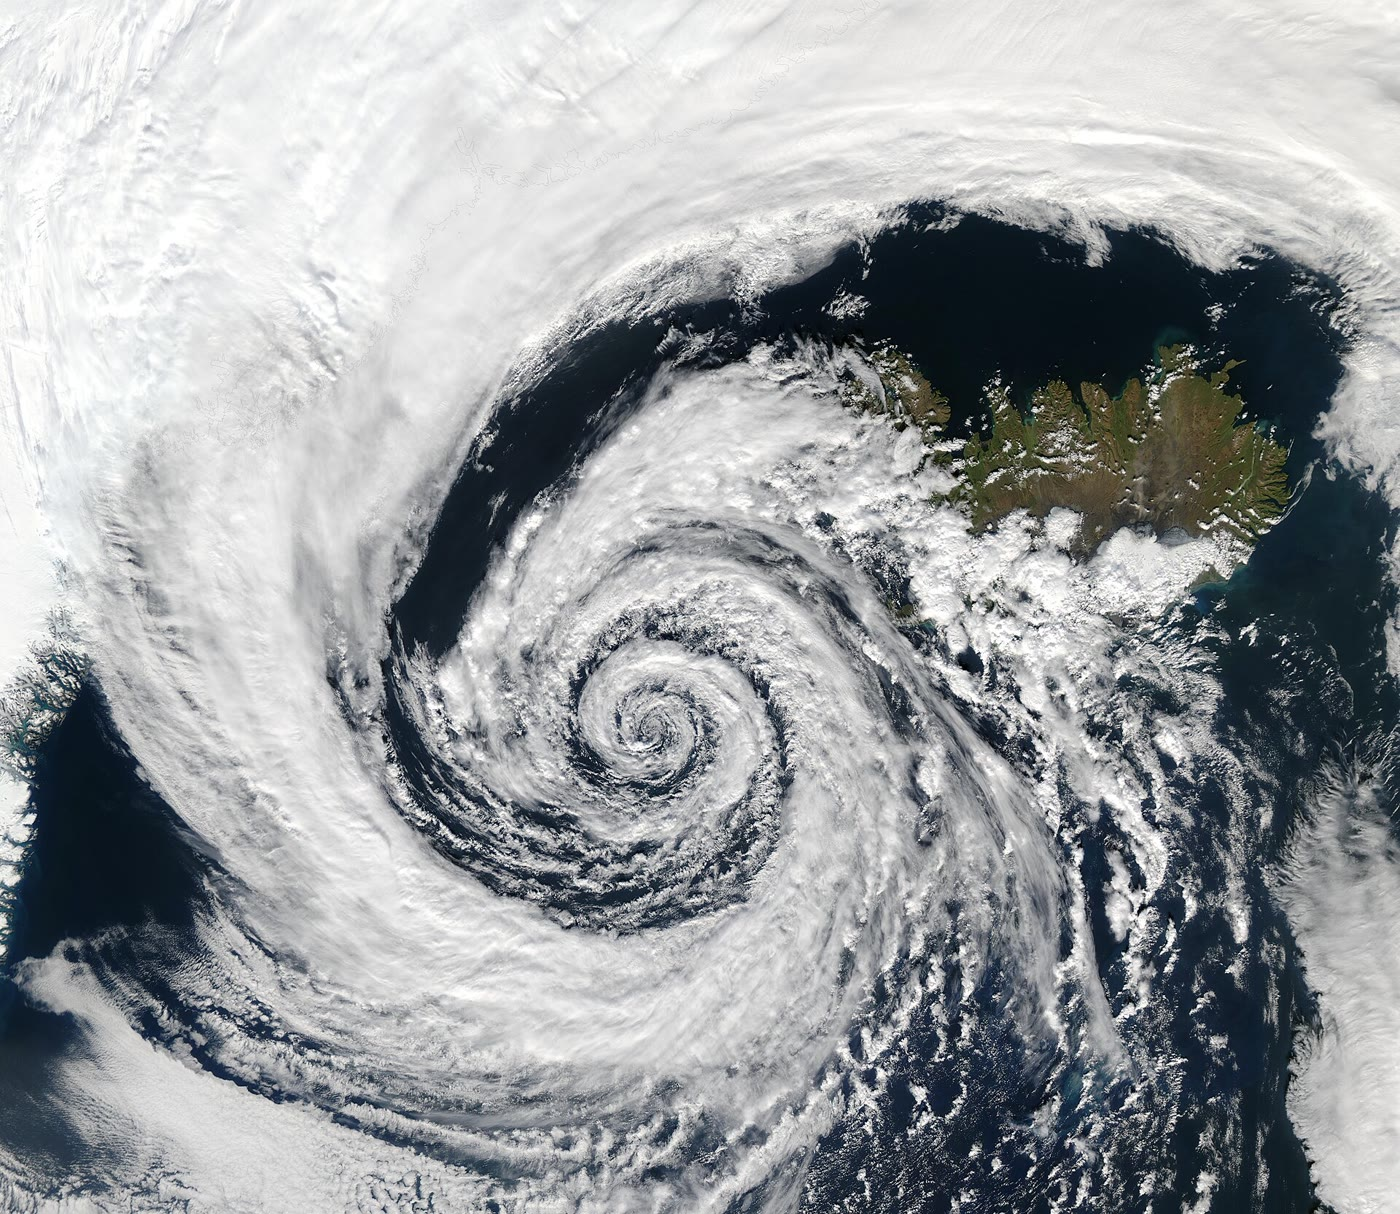
\includegraphics[width=0.58\linewidth]{images/book4/b2-22-iceland-low.jpg}
\par\smallskip{\small Una baja profunda frente a la costa suroeste de Islandia, el 4 de septiembre de 2003, vista por
el instrumento MODIS del satélite Aqua de la NASA: las bandas nubosas se enrollan en espiral hacia el centro. (NASA
Goddard Space Flight Center, MODIS Rapid Response Team, Jacques Descloitres, dominio público, a través de
Wikimedia Commons.)}
\end{omfigure}

\section{Las corrientes en chorro y las ondas de Rossby}\label{sec:b2:weather-systems:rossby}

Los ciclones no están repartidos al azar. El chorro polar, el núcleo rápido de los vientos del oeste por encima del
frente polar, acompaña la posición y el movimiento de las altas y las bajas de las latitudes
medias; es más rápido en sus máximos de viento (\textit{jet streaks}), los tramos donde su velocidad culmina, y
no rodea el polo como un anillo: serpentea.
% ledger: nws4:polar-front, nws4:jet-streak

\begin{definition}[Onda de Rossby; vaguada y dorsal en altura]\label{def:b2:weather-systems:rossby}
Una \emph{onda de Rossby}\index{onda de Rossby} es una onda del flujo del oeste de la troposfera alta,
una sucesión de vaguadas y dorsales de miles de kilómetros de longitud con una gran amplitud norte--sur.
Una \emph{vaguada en altura}\index{vaguada en altura} es una región alargada de presión relativamente baja
en una onda así, donde el flujo se curva hacia el ecuador; una \emph{dorsal en
altura}\index{dorsal en altura} es una región alargada de presión relativamente alta, donde se
curva hacia el polo.
\end{definition}
% ledger: nws4:rossby

Las \omterm{def:b2:weather-systems:rossby}{ondas de Rossby} existen porque el parámetro de Coriolis aumenta hacia el polo. El aire empujado hacia el polo
encuentra un $f$ mayor y, conservando su vorticidad absoluta, vuelve hacia el ecuador; el aire
empujado hacia el ecuador vuelve hacia el polo. El ritmo al que $f$ aumenta hacia el norte,
$\beta = \mathrm{d}f/\mathrm{d}y = 2\Omega\cos\varphi/a$ con $a$ el radio de la Tierra, fija
su velocidad. El volumen de tercer año deduce, a partir de la conservación de la vorticidad, la velocidad de fase de una
onda de longitud de onda $\lambda$ en un viento del oeste uniforme $U$:
\[
  c = U - \frac{\beta}{k^2}, \qquad k = \frac{2\pi}{\lambda} .
\]
Admítase aquí. Respecto del aire, toda \omterm{def:b2:weather-systems:rossby}{onda de Rossby} se desplaza hacia el oeste, y tanto más deprisa cuanto más larga es la
onda; el viento la lleva hacia el este. Las ondas cortas son arrastradas hacia el este casi a la velocidad del viento;
las largas derivan despacio, se quedan quietas o incluso se desplazan hacia el oeste.
% ledger: earth:Trot, earth:Rmean

\begin{example}[Tres ondas a 45° N]\label{ex:b2:weather-systems:rossby}
Con $\Omega = \qty{7.292e-5}{s^{-1}}$ (un día sidéreo de \qty{23.9345}{h}) y $a =
\qty{6371}{km}$, $\beta = \qty{1.62e-11}{m^{-1}.s^{-1}}$ a \ang{45} N. En un viento del oeste de
\qty{15}{m/s}, una onda de \qty{4000}{km} tiene $\beta/k^2 = \qty{6.6}{m/s}$ y se desplaza hacia el este a
\qty{8.4}{m/s}; una de \qty{6000}{km} tiene $\beta/k^2 = \qty{14.8}{m/s}$ y apenas se mueve, a
\qty{0.2}{m/s}; una de \qty{8000}{km} se desplaza hacia el oeste a \qty{11.2}{m/s}.
\end{example}
% ledger: earth:Trot, earth:Rmean

Las vaguadas de las ondas largas se desplazan despacio y duran mucho; las ondas cortas que viajan a través de
ellas, las vaguadas de onda corta, inducen aire ascendente por delante, en su lado este, donde la
presión en superficie baja y se forman bajas. Una vaguada cuyo eje se inclina de sureste a noroeste
suele ser signo de un sistema en formación o en intensificación.
% ledger: nws4:rossby

\begin{omfigure}
\centering
\begin{tikzpicture}[font=\scriptsize, >=Stealth]
\foreach \lat/\pa in {30/-72, 45/-72, 60/-108} {
  \pgfmathsetmacro{\r}{6.0*tan((90-\lat)/2)}
  \draw[black!25] (0,0) circle (\r);
  \node[black!50, fill=white, inner sep=1pt] at (\pa:\r) {\ang{\lat} N};
}
\fill (0,0) circle (0.6mm);
\node[anchor=north, black!60] at (0,-0.08) {Polo Norte};
\draw[ocBlue, very thick, smooth, samples=241, domain=0:360]
  plot ({6.0*tan((90-(47+11*cos(5*\x)))/2)*cos(\x)}, {6.0*tan((90-(47+11*cos(5*\x)))/2)*sin(\x)});
\foreach \a in {18, 90, 162, 234, 306} {
  \pgfmathsetmacro{\ra}{6.0*tan((90-(47+11*cos(5*\a)))/2)}
  \pgfmathsetmacro{\rb}{6.0*tan((90-(47+11*cos(5*(\a+2))))/2)}
  \draw[ocBlue, very thick, -{Stealth[length=2.6mm]}] (\a:\ra) -- (\a+2:\rb);
}
\pgfmathsetmacro{\rt}{6.0*tan((90-36)/2)}
\node[anchor=216, ocRed!80!black, inner sep=2pt] at (36:\rt) {vaguada};
\node[anchor=0, ocRed!80!black, inner sep=2pt] at (180:\rt) {vaguada};
\pgfmathsetmacro{\rr}{6.0*tan((90-58)/2)}
\node[anchor=72, ocRed!80!black, inner sep=3pt] at (72:\rr) {dorsal};
\end{tikzpicture}
\par\smallskip{\small \omterm{def:b2:weather-systems:rossby}{Ondas de Rossby} en la corriente en chorro vistas desde encima del Polo Norte (esquema):
cinco ondas alrededor del hemisferio, con vaguadas que se extienden hacia el ecuador y dorsales hacia el
polo. El chorro fluye hacia el este, en sentido antihorario visto desde encima del polo (flechas). Círculos de latitud
dibujados como en un mapa estereográfico polar.}
\end{omfigure}
% ledger: nws4:rossby

A veces la configuración deja de moverse por completo.

\begin{definition}[Bloqueo atmosférico]\label{def:b2:weather-systems:blocking}
El \emph{bloqueo atmosférico}\index{bloqueo atmosferico@bloqueo atmosférico} es un sistema de altas presiones grande, persistente y casi
estacionario, a veces emparejado con una baja, que interrumpe el flujo normal hacia el este
de la corriente en chorro. Los métodos de detección de bloqueos exigen casi todos que dure al menos cinco
días.
\end{definition}
% ledger: wang26:blocking

Un bloqueo desvía el chorro y los ciclones a su alrededor y mantiene el mismo tiempo sobre la misma
región durante días: los bloqueos traen olas de calor, sequías, incendios forestales, olas de frío e inundaciones a las
latitudes medias. A finales de junio y principios de julio de 2021, un fuerte bloqueo provocó la ola de calor del
Noroeste del Pacífico de América del Norte, que causó más de mil muertes. Los procesos físicos
que hay detrás del bloqueo todavía no se comprenden bien, y los modelos numéricos tienen dificultades para
reproducir la frecuencia con que se producen los bloqueos y su duración.
% ledger: wang26:blocking, wang26:gaps

\section{Los ciclones tropicales}\label{sec:b2:weather-systems:tropical}

Los ciclones tropicales no tienen frentes ni contraste de temperatura del que alimentarse. Obtienen su energía
del océano cálido, a través del calor latente del agua que evaporan, tal como lo midió el \cref{ch:b2:atmospheric-thermodynamics}.
Seis condiciones favorecen su formación: agua oceánica de al menos \qty{26.5}{\celsius}
en un espesor del orden de \qty{50}{m}; una atmósfera que se enfríe lo bastante deprisa con la altura para
ser inestable para la convección húmeda; una troposfera media húmeda, hacia \qty{5}{km}; una distancia de
al menos unos \qty{500}{km} al ecuador, para que la fuerza de Coriolis pueda mantener la baja en
equilibrio; una perturbación preexistente cerca de la superficie; y una cizalladura vertical del viento débil, por debajo de unos
\qty{10}{m/s} entre la superficie y la troposfera alta. Son necesarias pero no
suficientes: muchas perturbaciones que las cumplen nunca se desarrollan.
% ledger: aoml:tc-genesis

Una vez formado, un ciclón tropical es una máquina térmica. El aire converge en espiral hacia el centro sobre el mar a temperatura casi
constante, ganando calor y humedad del océano; en la pared del ojo asciende
adiabáticamente; en la salida cerca de la tropopausa pierde calor por radiación a una temperatura baja,
casi constante; y desciende de nuevo lejos del centro, completando un ciclo que
se parece al de Carnot. El trabajo del ciclo mueve los vientos contra el rozamiento de la superficie
del mar.
% ledger: gilford21:pi

\begin{omfigure}
\centering
\begin{tikzpicture}[font=\scriptsize, >=Stealth, x=1cm, y=1cm]
% sea and axis
\fill[ocBlue!12] (0,-0.35) rectangle (12.5,0);
\draw[thick, ocBlue!70!black] (0,0) -- (12.5,0);
\node[anchor=north west, ocBlue!70!black] at (8.6,-0.02) {mar cálido, $T_s$};
\draw[dashed, black!50] (0,-0.35) -- (0,4.9);
\node[anchor=south, black!60] at (0,4.9) {centro};
% eyewall cloud and outflow cloud
\fill[black!14, draw=black!40] (0.9,0.25) .. controls (0.7,1.8) and (0.75,3.3) .. (0.95,4.2)
  .. controls (3.5,4.55) and (7.0,4.45) .. (9.5,4.2) .. controls (7.0,3.9) and (3.6,3.85)
  .. (2.1,3.7) .. controls (1.95,2.6) and (1.9,1.4) .. (2.0,0.25) -- cycle;
\node[black!60] at (0.45,2.0) [rotate=90] {ojo};
\draw[black!50] (1.9,1.1) -- (2.45,1.1) node[anchor=west, black!70] {nube de la pared del ojo};
% the cycle
\draw[->, very thick, ocRed] (11.4,0.3) -- (2.3,0.3);
\draw[->, very thick, ocRed] (1.45,0.45) .. controls (1.4,1.6) and (1.45,3.0) .. (1.75,4.0);
\draw[->, very thick, ocBlue] (2.2,4.25) -- (11.2,4.25);
\draw[->, very thick, ocBlue] (11.6,4.05) .. controls (11.75,2.8) and (11.75,1.5) .. (11.6,0.45);
\fill (11.6,0.3) circle (0.7mm) node[right=2pt] {A};
\fill (1.45,0.3) circle (0.7mm) node[left=2pt] {B};
\fill (1.8,4.25) circle (0.7mm) node[above left=1pt] {C};
\fill (11.6,4.25) circle (0.7mm) node[above right=1pt] {D};
\node[anchor=south, align=center] at (6.5,0.35) {A$\to$B: entrada sobre el mar a unos $T_s$,
  tomando calor y humedad};
\node[anchor=west, align=left] at (2.25,2.3) {B$\to$C: asciende en la pared del ojo,\\sin
  intercambiar calor (adiabática húmeda)};
\node[anchor=south, align=center] at (6.5,4.62) {C$\to$D: salida cerca de la tropopausa a unos
  $T_o$, perdiendo calor por radiación};
\node[anchor=east, align=right] at (11.45,2.3) {D$\to$A: desciende lejos\\del centro};
\end{tikzpicture}
\par\smallskip{\small La máquina térmica de un ciclón tropical, en un corte vertical desde el centro
hacia fuera (esquema, sin escala): el calor se toma a la temperatura de la superficie del mar
(A$\to$B) y se cede a la temperatura, mucho más baja, de la salida (C$\to$D), como en un ciclo de
Carnot.}
\end{omfigure}
% ledger: gilford21:pi

\begin{proposition}[Intensidad potencial]\label{prop:b2:weather-systems:pi}
\index{intensidad potencial}
La \emph{\omterm{prop:b2:weather-systems:pi}{intensidad potencial}} de un ciclón tropical, la velocidad máxima del viento cerca de la superficie que
el océano y la atmósfera que lo rodean pueden mantener, viene dada aproximadamente por
\[
  V_{\max}^2 = \frac{C_k}{C_D}\,\frac{T_s - T_o}{T_o}\,\bigl(h_o^* - h^*\bigr),
\]
donde $T_s$ es la temperatura de la superficie del mar, $T_o$ la temperatura de la salida, $C_k/C_D$
el cociente de los coeficientes de intercambio de entalpía y de cantidad de movimiento entre el mar y el aire,
que suele tomarse igual a 0.9, y $h_o^* - h^*$ el exceso de $c_pT + gz + Lq$ en la saturación en la superficie
del mar sobre su valor de saturación en el aire por encima de la capa límite (se admite).
\end{proposition}
% ledger: gilford21:pi

La fracción $(T_s - T_o)/T_o$ no es el rendimiento de Carnot $(T_s - T_o)/T_s$ de los libros de
física: es mayor en el factor $T_s/T_o$, porque el rozamiento que disipa el trabajo calienta
el aire que entra cerca de la superficie del mar, y la máquina vuelve a usar ese calor. El último
factor es el combustible. En una atmósfera tropical cuya temperatura sigue la \omterm{def:b2:atmospheric-thermodynamics:moist-adiabat}{adiabática húmeda} del aire de su
capa límite, $h^*$ es el valor de $c_pT + gz + Lq$ en ese aire, y $h_o^* - h^*$
mide lo lejos que está el aire sobre el mar de la saturación a la temperatura del mar:
\[
  h_o^* - h^* \approx c_p\,(T_s - T_a) + L\,(q_s^* - q_a),
\]
con $T_a$ y $q_a$ la temperatura y la \omterm{def:b2:atmospheric-thermodynamics:moist-air}{humedad específica} del aire cerca de la superficie y
$q_s^*$ la \omterm{def:b2:atmospheric-thermodynamics:moist-air}{humedad específica} de saturación a la temperatura de la superficie del mar.
% ledger: gilford21:pi

\begin{example}[Una intensidad potencial]\label{ex:b2:weather-systems:pi}
Sobre un mar a \qty{29}{\celsius}, el aire a \qty{1015}{hPa} está a \qty{28}{\celsius} con una
humedad relativa del \qty{80}{\percent}, y la salida está a \qty{200}{K}, una media anual típica
sobre los océanos tropicales cálidos. Por la \cref{prop:b2:atmospheric-thermodynamics:es,prop:b2:atmospheric-thermodynamics:humidity},
$e_s(\qty{29}{\celsius}) = \qty{41.0}{hPa}$, así que $q_s^* = \qty{25.5}{g/kg}$, y el aire, con
$e = 0.8 \times \qty{38.7}{hPa}$, tiene $q_a = \qty{19.2}{g/kg}$. Entonces $h_o^* - h^* = 1004.5 \times
1 + 2.501 \times 10^6 \times 0.0063 = \qty{16.8}{kJ/kg}$, el factor $(T_s - T_o)/T_o$ es
$(302.15 - 200)/200 = 0.511$, y $V_{\max} = \sqrt{0.9 \times 0.511 \times 16\,800} =
\qty{88}{m/s}$.
\end{example}
% ledger: gilford21:pi

Las tormentas más fuertes se acercan a esos valores: lo más alto de la escala de Saffir--Simpson, la categoría
5, empieza en \qty{70}{m/s}, y cinco tormentas recientes han superado los \qty{86}{m/s}. La mayoría de las tormentas
rara vez alcanzan su \omterm{prop:b2:weather-systems:pi}{intensidad potencial}: las tormentas reales casi nunca están en el estado estacionario que supone
la teoría, y la teoría deja fuera la cizalladura vertical del viento, el aire seco que entra en la tormenta y el
descenso del aire que la rodea, que debilitan una tormenta.
% ledger: wk24:scale, gilford21:limits, aoml:tc-weaken

\begin{omfigure}
\centering
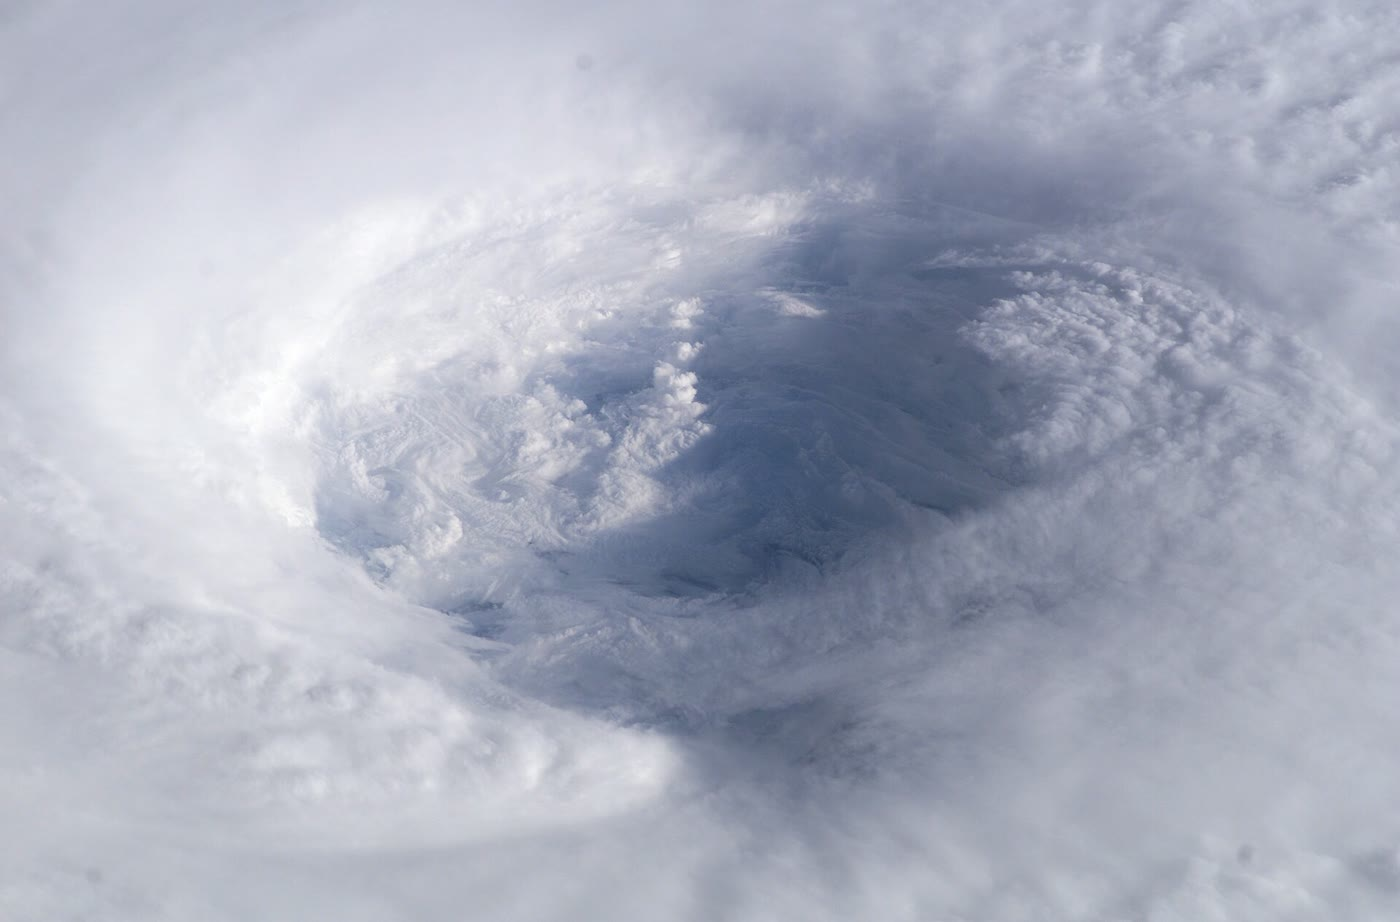
\includegraphics[width=0.62\linewidth]{images/book4/b2-22-isabel-eye.jpg}
\par\smallskip{\small El ojo del huracán Isabel, el 13 de septiembre de 2003, fotografiado desde la
Estación Espacial Internacional: la pared del ojo cae como las gradas de un estadio hasta las nubes bajas del ojo.
(Astronauta de la NASA Ed Lu, dominio público, a través de Wikimedia Commons.)}
\end{omfigure}

\section{La predicción numérica del tiempo}\label{sec:b2:weather-systems:nwp}

\begin{definition}[Predicción numérica del tiempo; asimilación de datos; predicción por conjuntos; límite de predictibilidad]\label{def:b2:weather-systems:nwp}
La \emph{predicción numérica del tiempo}\index{prediccion numerica del tiempo@predicción numérica del tiempo} es la predicción por
ordenador: las ecuaciones que rigen el movimiento, la energía y el agua de la atmósfera se
integran hacia delante en el tiempo a partir de su estado observado. La \emph{asimilación de datos}\index{asimilacion de datos@asimilación de datos}
combina las observaciones más recientes con una predicción a corto plazo hecha a partir de observaciones
anteriores para obtener la mejor estimación del estado presente, el análisis, del que parte la
predicción. Una \emph{predicción por conjuntos}\index{prediccion por conjuntos@predicción por conjuntos} es un conjunto de predicciones lanzadas
desde estados iniciales ligeramente distintos, y con versiones ligeramente distintas del modelo, para
mostrar el abanico de tiempos posibles y su probabilidad. El \emph{límite de
predictibilidad}\index{limite de predictibilidad@límite de predictibilidad} es el plazo más allá del cual una predicción del estado del
tiempo no es mejor que una conjetura basada en el clima, porque los errores del estado inicial han
crecido hasta igualar las diferencias entre dos estados cualesquiera de la atmósfera.
\end{definition}
% ledger: nws4:nwp, ecmwf4:da, ecmwf4:ens-fs, krish19:predictability

La primera predicción numérica se calculó en 1950 en el ENIAC, uno de los primeros ordenadores
electrónicos. Un modelo global divide hoy la atmósfera en una malla de celdas de unos pocos kilómetros
de lado y parte de un análisis que combina observaciones de estaciones meteorológicas, aviones,
radiosondas, barcos, boyas y, sobre todo, satélites, que aportan la mayor contribución a la
calidad de las predicciones globales. En un gran centro de predicción el conjunto
tiene 51 miembros, una pasada de control y 50 perturbadas, con una resolución de unos \qty{9}{km}, lanzadas
dos veces al día hasta 15 días vista.
% ledger: krish19:predictability, ecmwf4:da, ecmwf4:ens

¿Por qué perturbar una predicción que podría partir del mejor análisis? Porque la atmósfera es
caótica, sensible a su estado inicial. Un sistema de tres variables, publicado en 1963, lo muestra
a la escala más pequeña.

\begin{proposition}[El sistema de Lorenz]\label{prop:b2:weather-systems:lorenz}
El sistema
\[
  \dot x = \sigma(y - x), \qquad \dot y = x(r - z) - y, \qquad \dot z = xy - bz,
\]
con $\sigma = 10$, $r = 28$ y $b = 8/3$, tiene las propiedades siguientes.
\begin{enumerate}
  \item Sus puntos fijos son el origen y $C_\pm = \bigl(\pm\sqrt{b(r - 1)}, \pm\sqrt{b(r - 1)},
        r - 1\bigr) = (\pm 8.49, \pm 8.49, 27)$.
  \item Todo volumen de su espacio de fases se contrae como $\mathrm{e}^{-(\sigma + 1 + b)t}$: sus
        trayectorias acaban en un conjunto de volumen nulo, el atractor.
  \item Sobre el atractor, dos trayectorias que parten a una pequeña distancia $\delta_0$ se separan,
        en promedio, como $\delta(t) \approx \delta_0\,\mathrm{e}^{\lambda t}$, con $\lambda =
        0.906$, hasta que $\delta$ alcanza el tamaño del atractor (calculado, se admite). Los errores
        pequeños se duplican cada $\ln 2/\lambda = 0.77$ unidades de tiempo.
\end{enumerate}
\end{proposition}
% ledger: nolitia22:lorenz

\begin{proof}[Demostración de 1 y 2]
En un punto fijo, $y = x$ por la primera ecuación; la tercera da $z = x^2/b$; la segunda
se convierte en $x(r - 1 - x^2/b) = 0$, así que $x = 0$ o $x^2 = b(r - 1) = 72$. La divergencia del
campo vectorial es $\partial_x\dot x + \partial_y\dot y + \partial_z\dot z = -\sigma - 1 - b$, una
constante, y por el teorema de la divergencia un volumen $V$ transportado por el flujo cumple $\dot V =
-(\sigma + 1 + b)V$.
\end{proof}

Las figuras muestran lo que significa la proposición. Dos pasadas que parten a \num{e-5} de distancia se siguen
durante unas quince unidades de tiempo, y después se separan para siempre: cada una sigue pareciendo una trayectoria
plausible del sistema, pero ya no son la misma trayectoria. Promediada sobre 200 pares de
pasadas iniciadas a \num{e-8} de distancia, la distancia crece exponencialmente al ritmo $\lambda$, una recta
en escala logarítmica, hasta saturarse en el tamaño del atractor. Sea cual sea el
error inicial, alcanza ese tamaño: un error inicial menor solo retrasa el momento, en
$\ln 10/\lambda = 2.5$ unidades de tiempo por cada reducción a la décima parte.
% ledger: nolitia22:lorenz

\begin{omfigure}
\centering
% figdata/bachelor-2/weather.py parts traj, butterfly
\begin{tikzpicture}
\begin{groupplot}[group style={group size=2 by 1, horizontal sep=1.5cm},
  tick label style={font=\scriptsize}, label style={font=\small}]
\nextgroupplot[width=0.58\linewidth, height=5.0cm, xmin=0, xmax=30, ymin=-22, ymax=22,
  xlabel={tiempo}, ylabel={$x$}, legend style={font=\scriptsize, at={(0.5,1.02)},
  anchor=south, draw=none, legend columns=2, /tikz/every even column/.append style={column
  sep=0.4cm}}, legend cell align=left]
\addplot[ocBlue, thin] table[x=t, y=x1] {figdata/out/bachelor-2-weather-traj.dat};
\addlegendentry{pasada 1}
\addplot[ocRed, thin, densely dashed] table[x=t, y=x2] {figdata/out/bachelor-2-weather-traj.dat};
\addlegendentry{pasada 2, iniciada a \num{e-5}}
\nextgroupplot[width=0.4\linewidth, height=5.0cm, xmin=-22, xmax=22, ymin=0, ymax=52,
  xlabel={$x$}, ylabel={$z$}]
\addplot[black!70, very thin] table[x=x, y=z] {figdata/out/bachelor-2-weather-butterfly.dat};
\addplot[only marks, mark=*, mark size=1.3pt, ocRed] coordinates {(8.485,27) (-8.485,27)};
\end{groupplot}
\end{tikzpicture}
\par\smallskip{\small El sistema de Lorenz ($\sigma = 10$, $r = 28$, $b = 8/3$), integrado por el
método de Runge--Kutta con un paso de tiempo de 0.01. Izquierda: dos pasadas que parten a \num{e-5} de distancia en $x$
sobre el atractor. Derecha: una pasada de 40 unidades de tiempo, vista a lo largo de $y$, con los puntos fijos
$C_\pm$ (en rojo).}
\end{omfigure}
% ledger: nolitia22:lorenz

\begin{omfigure}
\centering
% figdata/bachelor-2/weather.py part growth
\begin{tikzpicture}
\begin{axis}[width=0.72\linewidth, height=5.6cm, xmin=0, xmax=30, ymode=log, ymin=1e-9,
  ymax=1e3, ytick={1e-9,1e-7,1e-5,1e-3,1e-1,1e1,1e3}, xlabel={tiempo}, ylabel={distancia entre las pasadas}, tick label style={font=\scriptsize},
  label style={font=\small}, legend style={font=\scriptsize, at={(0.02,0.98)}, anchor=north west,
  draw=none, fill=none}, legend cell align=left, unbounded coords=discard, grid=major,
  grid style={black!8}]
\addplot[ocBlue, line width=1.6pt, opacity=0.55] table[x=t, y expr=10^\thisrow{log10d}]
  {figdata/out/bachelor-2-weather-growth.dat};
\addlegendentry{media de 200 pares (geométrica)}
\addplot[black, densely dashed, thin] table[x=t, y expr=10^\thisrow{fit}]
  {figdata/out/bachelor-2-weather-growth.dat};
\addlegendentry{exponencial ajustada, $t = 2$ a 16}
\end{axis}
\end{tikzpicture}
\par\smallskip{\small Crecimiento de la distancia entre pares de pasadas del sistema de Lorenz iniciadas
a \num{e-8} de distancia. La recta ajustada se multiplica por diez cada 2.57 unidades de tiempo, un ritmo de 0.897;
el mayor exponente de Lyapunov, calculado renormalizando un único par a lo largo de 2000 unidades de tiempo, es
0.909, frente a los 0.906 publicados. El crecimiento se detiene en el tamaño del atractor.}
\end{omfigure}
% ledger: nolitia22:lorenz

La atmósfera se comporta de la misma manera, con muchas más variables y con errores que crecen a
ritmos distintos en escalas distintas. A partir de las predicciones de la década de 1980 se halló que los errores pequeños
se duplicaban en unos 2.4 días, y la predicción fiable del estado del tiempo se detiene antes de
unos diez días. Los experimentos que reducen la incertidumbre actual del estado inicial, con un modelo
supuesto perfecto, encuentran que unas condiciones iniciales perfectas solo añadirían de cuatro a cinco días, y
que una reducción del 90 por ciento ya da casi todo ese margen: a medida que los errores se hacen más pequeños, crecen
más deprisa, por la liberación de calor latente en la convección, en escalas más pequeñas de las que la predicción
puede resolver. El \omterm{def:b2:weather-systems:nwp}{límite de predictibilidad} de las latitudes medias se sitúa en torno a dos semanas. Las predicciones
ganan aproximadamente un día por década porque unas observaciones, una asimilación y unos modelos mejores las acercan
a ese límite; no pueden cruzarlo.
% ledger: krish19:predictability, selz22:limit, bauer:day-per-decade

El conjunto convierte esto en una herramienta. Sus miembros parten de análisis que difieren aproximadamente tanto
como es incierto el propio análisis; mientras coinciden, la predicción es nítida; cuando se
dispersan, la predicción debe decirlo, y da probabilidades. Una predicción se llama fiable cuando
los sucesos que anuncia con una probabilidad del \qty{70}{\percent} ocurren en el \qty{70}{\percent} de
los casos.
% ledger: ecmwf4:ens-fs

\begin{inthelab}[Un día en un centro de predicción]
\begin{minipage}[t]{0.54\linewidth}\vspace{0pt}
En un centro de predicción global el día gira en torno a dos horas, las 00 y las 12 UTC. Las observaciones válidas
en torno a cada hora llegan por millones, de satélites, radiosondas, aviones, barcos,
boyas y estaciones meteorológicas; la \omterm{def:b2:weather-systems:nwp}{asimilación de datos} las combina con la predicción corta anterior en
el análisis. Los modelos parten de él, el conjunto también, y las predicciones llegan a sus usuarios
varias horas después, cuando los superordenadores han calculado los 15 días siguientes. Los predictores
comparan entonces las pasadas, las contrastan con las últimas observaciones y las imágenes de satélite, siguen
los ciclones y los frentes, y convierten las probabilidades del conjunto en avisos y
predicciones.
\end{minipage}\hfill
\begin{minipage}[t]{0.42\linewidth}\vspace{0pt}
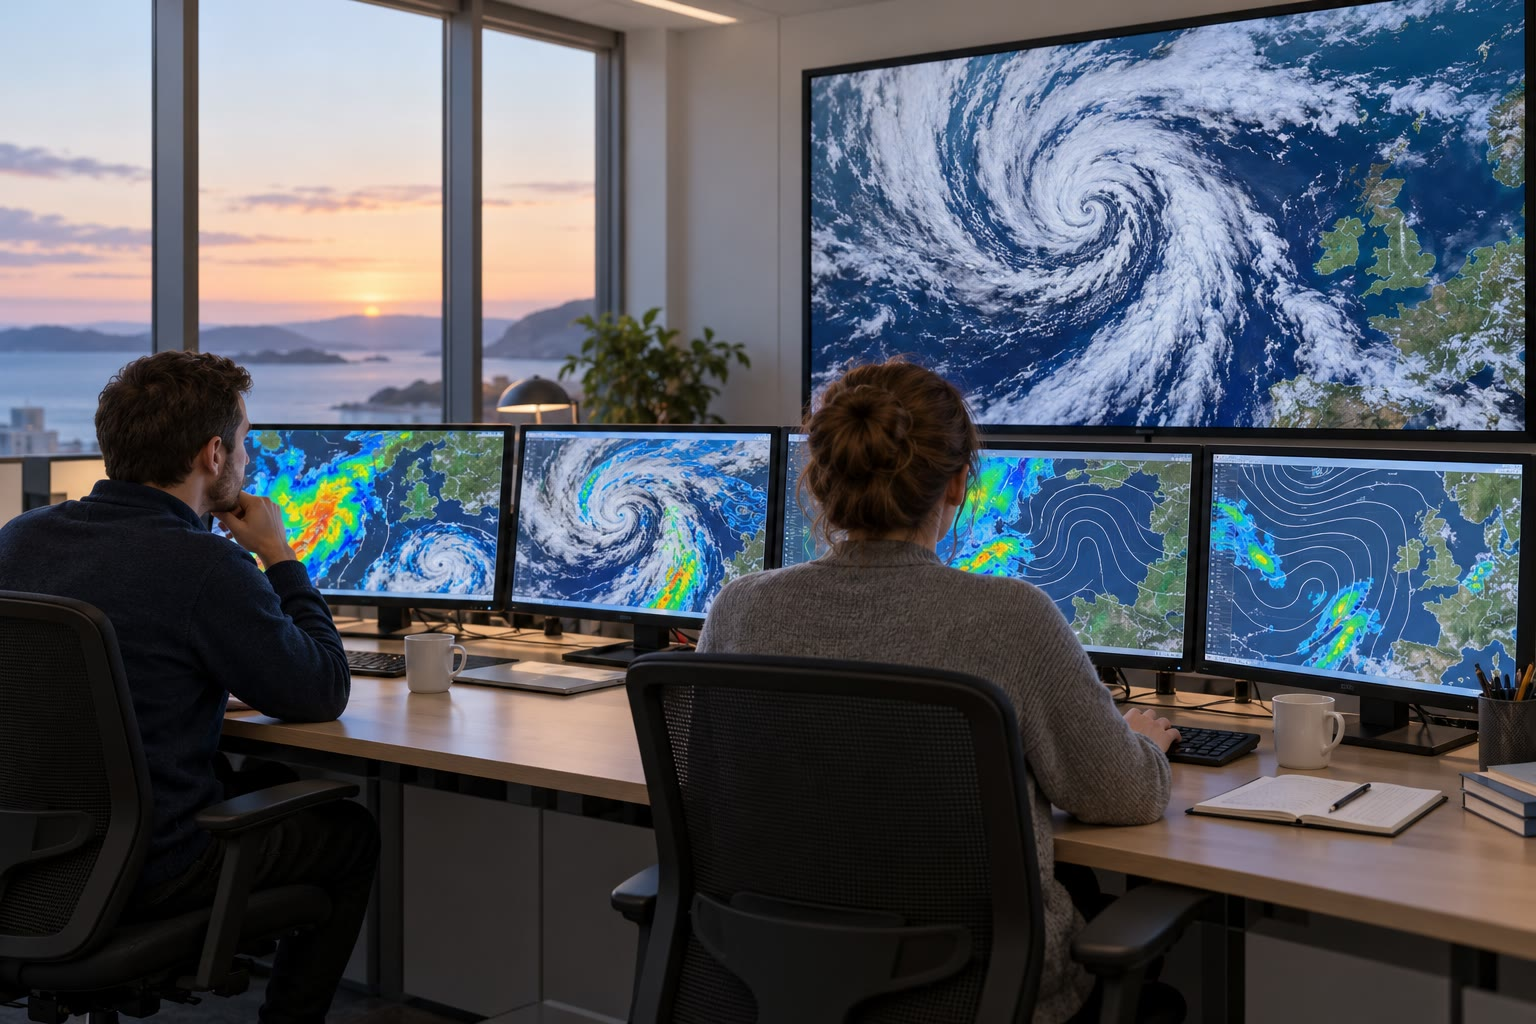
\includegraphics[width=\linewidth]{images/book4/ai/b2-forecast-office.jpg}

{\scriptsize Predictores trabajando ante imágenes de satélite y mapas de los modelos
(ilustración generada por IA).}
\end{minipage}
% ledger: ecmwf4:ens, ecmwf4:da, mo:how-forecasts
\end{inthelab}

\section*{Ejercicios}\label{sec:b2:weather-systems:exercises}

Datos de los ejercicios, salvo aviso contrario: $\Omega = \qty{7.292e-5}{s^{-1}}$, $a =
\qty{6371}{km}$, $g = \qty{9.81}{m.s^{-2}}$, $c_p = \qty{1004.5}{J.kg^{-1}.K^{-1}}$, $L =
\qty{2.501e6}{J/kg}$, y la \omterm{def:b2:atmospheric-thermodynamics:moist-air}{presión de vapor} de saturación de los ejercicios del
\cref{ch:b2:atmospheric-thermodynamics}.
% ledger: earth:Trot, earth:Rmean

\begin{exercise}[$\star$]\label{exo:b2:weather-systems:1}
A \ang{50} N un frente frío separa aire a \qty{275}{K} de aire a \qty{281}{K}, y el viento
a lo largo de él cambia \qty{15}{m/s}. (a) Calcúlese $f$. (b) Calcúlese la pendiente de la \omterm{def:b2:weather-systems:fronts}{superficie frontal},
en la forma 1 por cada $N$. (c) ¿A qué distancia por detrás del frente en el suelo alcanza la \omterm{def:b2:weather-systems:fronts}{superficie frontal}
\qty{1}{km}? (d) ¿Qué le ocurre a la pendiente si el contraste de temperatura se duplica con el mismo salto
de viento?
\end{exercise}

\begin{exercise}[$\star$]\label{exo:b2:weather-systems:2}
Una \omterm{def:b2:weather-systems:fronts}{superficie frontal} cálida se eleva con una pendiente de 1 por cada 150 y avanza a \qty{25}{km/h}. (a) ¿A qué distancia por delante del
frente en el suelo está la \omterm{def:b2:weather-systems:fronts}{superficie frontal} a \qty{6}{km} de altura? (b) Un observador ve formarse nubes altas
sobre ella allí. ¿Cuánto tiempo después llega el frente al observador? (c) Descríbase la sucesión de
nubes que el observador ve entretanto.
\end{exercise}
% ledger: ucar:warm-front

\begin{exercise}[$\star$]\label{exo:b2:weather-systems:3}
En un mapa del hemisferio norte, (a) una línea con triángulos azules en su lado sureste va hacia el suroeste
desde una baja; (b) una línea con semicírculos rojos en su lado norte va hacia el este desde la misma baja; (c) una
línea violeta con ambos símbolos va desde otra baja hasta un punto donde empiezan otros dos frentes;
(d) una línea alterna triángulos azules en su lado sur y semicírculos rojos en su lado norte.
Nómbrese cada frente, dígase dónde está el aire frío y hacia dónde se mueve cada uno.
\end{exercise}
% ledger: ucar4:stationary-occluded, nws4:occluded

\begin{exercise}[$\star$]\label{exo:b2:weather-systems:4}
A \ang{45} N en un viento del oeste de \qty{12}{m/s}: (a) calcúlese $\beta$. (b) Calcúlese la velocidad de fase
de ondas de \qty{4000}{km} y \qty{8000}{km}. (c) ¿Hacia dónde se mueve cada una, y cuánto en un
día?
\end{exercise}

\begin{exercise}[$\star\star$]\label{exo:b2:weather-systems:5}
(a) Demuéstrese que una \omterm{def:b2:weather-systems:rossby}{onda de Rossby} se queda quieta en un viento del oeste $U$ cuando $\lambda = 2\pi\sqrt{U/\beta}$.
(b) Calcúlese a \ang{45} N para $U = \qty{12}{m/s}$. (c) ¿Cuántas ondas así caben alrededor del
círculo de latitud? (d) ¿Por qué un viento del oeste más fuerte favorecería ondas estacionarias menos numerosas y más largas?
\end{exercise}

\begin{exercise}[$\star\star$]\label{exo:b2:weather-systems:6}
Para el sistema de Lorenz: (a) compruébese que $C_+$ es un punto fijo calculando allí las tres derivadas.
(b) ¿En qué factor se contrae un pequeño volumen del espacio de fases en una unidad de tiempo? (c) ¿Por qué
no impide esto que dos trayectorias próximas se separen?
\end{exercise}

\begin{exercise}[$\star\star$]\label{exo:b2:weather-systems:7}
Tómense $\lambda = 0.906$ para el sistema de Lorenz y un atractor de tamaño 10. (a) Calcúlese el
tiempo de duplicación de los errores pequeños. (b) ¿Cuánto tarda un error de \num{e-8} en alcanzar el tamaño del
atractor? (c) ¿Cuánto retrasa ese momento un error inicial mil veces menor? ¿Qué
fracción del tiempo hallado en (b) representa?
\end{exercise}
% ledger: nolitia22:lorenz

\begin{exercise}[$\star\star$]\label{exo:b2:weather-systems:8}
Un mar a \qty{303}{K} tiene una salida a \qty{195}{K}; el desequilibrio es $h_o^* - h^* =
\qty{15}{kJ/kg}$ y $C_k/C_D = 0.9$. (a) Calcúlese la \omterm{prop:b2:weather-systems:pi}{intensidad potencial}. (b) Compárese con
el umbral de la categoría 5 y con las tormentas recientes más rápidas. (c) ¿Por qué la mayoría de las tormentas no la
alcanzan?
\end{exercise}
% ledger: gilford21:pi, wk24:scale

\begin{exercise}[$\star\star$]\label{exo:b2:weather-systems:9}
Para la tormenta del \cref{exo:b2:weather-systems:8}: (a) calcúlese el rendimiento de Carnot de una máquina
que funcione entre la superficie del mar y la salida. (b) Calcúlense el factor $(T_s - T_o)/T_o$ de la
\cref{prop:b2:weather-systems:pi} y el cociente de ambos. (c) Explíquese la diferencia.
\end{exercise}
% ledger: gilford21:pi

\begin{exercise}[$\star\star\star$]\label{exo:b2:weather-systems:10}
(a) Vuélvase a deducir la \cref{prop:b2:weather-systems:slope} conservando las densidades exactas, y demuéstrese que
el aire frío debe estar debajo. (b) A través de una zona frontal de \qty{50}{km} de anchura a \ang{45} N, el viento
a lo largo del frente cambia \qty{10}{m/s}. Calcúlese la vorticidad relativa de la zona y compárese
con $f$. (c) ¿Es la zona ciclónica o anticiclónica?
\end{exercise}

\begin{exercise}[$\star\star\star$]\label{exo:b2:weather-systems:11}
Supóngase que los errores de predicción se duplican cada 2.4 días, empiezan en \qty{0.5}{K} y hacen inútil la predicción a
\qty{6}{K}. (a) Hállese el horizonte de las predicciones útiles. (b) ¿En qué factor debe
reducirse el error inicial cada década para ganar un día por década, si el modelo fuera perfecto? (c) Los experimentos encuentran que
un error inicial diez veces menor solo gana de 4 a 5 días. ¿Qué tiempo de duplicación implica eso para los
errores pequeños, y qué dice sobre cómo crecen los errores pequeños?
\end{exercise}
% ledger: krish19:predictability, selz22:limit, bauer:day-per-decade

\begin{exercise}[$\star\star\star$]\label{exo:b2:weather-systems:12}
Tómese el \cref{ex:b2:weather-systems:pi} y caliéntense el mar y el aire \qty{1}{K}, con la
humedad relativa y la temperatura de la salida sin cambios. (a) Vuélvanse a calcular $q_s^*$, $q_a$ y el
desequilibrio. (b) Vuélvase a calcular la \omterm{prop:b2:weather-systems:pi}{intensidad potencial}. (c) ¿En qué tanto por ciento por kelvin
aumenta, y qué factor contribuye más?
\end{exercise}
% ledger: gilford21:pi

\begin{problem}[{Problema de fin de semana --- ¿Con cuánta antelación?}]\label{pb:b2:weather-systems:1}
Un mapa meteorológico inventado a \ang{50} N muestra un frente frío que avanza hacia una ciudad, con una \omterm{def:b2:weather-systems:rossby}{onda de
Rossby} en la corriente en chorro por encima. El problema sigue el frente, luego la onda, y después pregunta con cuánta
antelación puede predecirse todo ello. Úsense los datos de los ejercicios.

\medskip\noindent\textbf{Parte I --- El frente.}
A las 06 UTC el frente frío está a \qty{480}{km} al oeste de la ciudad, a las 12 UTC a \qty{390}{km}. Por detrás
el aire está a \qty{277}{K}, en el sector cálido a \qty{285}{K}, y el viento a lo largo del frente
cambia \qty{16}{m/s} a través de él.
\begin{enumerate}
  \item Hállese la velocidad del frente.
  \item ¿A qué hora llega a la ciudad?
  \item Calcúlese $f$ a \ang{50} N.
  \item Calcúlese la pendiente de la \omterm{def:b2:weather-systems:fronts}{superficie frontal}.
  \item ¿A qué altura está la \omterm{def:b2:weather-systems:fronts}{superficie frontal} sobre la ciudad seis horas después del paso del frente?
  \item ¿Cuánto tiempo después del paso alcanza el aire frío \qty{1.5}{km} sobre la ciudad?
  \item ¿Qué tiempo ve la ciudad al pasar el frente, y cómo cambia la presión?
\end{enumerate}

\medskip\noindent\textbf{Parte II --- La onda en altura.}
En el chorro, por encima, el viento del oeste es de \qty{20}{m/s} y la onda tiene una longitud de onda de \qty{5000}{km}.
\begin{enumerate}[resume]
  \item Calcúlese $\beta$ a \ang{50} N.
  \item Calcúlense $k$ y $\beta/k^2$.
  \item Hállese la velocidad de fase de la onda.
  \item ¿Cuánto se desplaza una vaguada en 24 horas?
  \item Hállense la longitud de onda que se quedaría quieta en este viento, y cuántas ondas así caben
        alrededor de \ang{50} N.
  \item ¿Dónde, respecto de la \omterm{def:b2:weather-systems:rossby}{vaguada en altura}, debería profundizarse el ciclón de superficie?
\end{enumerate}

\medskip\noindent\textbf{Parte III --- Una atmósfera de juguete.}
En la figura del crecimiento de los errores en el sistema de Lorenz, la recta ajustada pasa por
unos \num{5e-7} en $t = 4$ y \num{3.9e-3} en $t = 14$.
\begin{enumerate}[resume]
  \item A partir de estas dos lecturas, calcúlese el ritmo de crecimiento $\lambda$.
  \item Calcúlese el tiempo de duplicación.
  \item Compárese con el exponente publicado, 0.906.
  \item ¿Por qué la distancia deja de crecer, hacia 15?
  \item ¿Cuánto más tarde alcanza ese tamaño un error diez veces menor?
\end{enumerate}

\medskip\noindent\textbf{Parte IV --- ¿Con cuánta antelación?}
Tómense el tiempo de duplicación de 2.4 días hallado para los errores pequeños de las predicciones de la década de 1980, un
error inicial de \qty{0.1}{\celsius} en la temperatura en algún nivel, y una predicción que se vuelve
inútil cuando el error alcanza \qty{3}{\celsius}.
\begin{enumerate}[resume]
  \item ¿Cuántas duplicaciones separan el error inicial del error que inutiliza la predicción?
  \item ¿Cuántos días lleva eso?
  \item ¿Cuántos días ganaría reducir a la mitad el error inicial?
  \item Con la estimación anterior de un tiempo de duplicación de 5 días, ¿qué horizonte se hallaría?
  \item Los experimentos modernos encuentran que un error inicial diez veces menor, e incluso un estado
        inicial perfecto, solo gana de 4 a 5 días. ¿Por qué sugiere eso que la estimación de
        la pregunta 20 es optimista?
  \item En resumen: ¿con cuánta antelación, en días, podría ser útil esta predicción?
\end{enumerate}
\end{problem}
% ledger: krish19:predictability, selz22:limit, nolitia22:lorenz, ucar:cold-front
